\section{Problem 7 - K-means Clustering \& Principal Component Analysis}

% a) Provide a code snippet in the report showing how you perform the normalization
\subsection {a)}
I've decided to make my own function to normalize my data. It normalizes the input
value x by subtracting the mean and dividion by the standard deviation.
\begin{minted}[linenos, bgcolor = bg, breaklines]{python}
    def normalizeData(x):
    '''
    Normalizes the input using mean and the standard deviation.
    Normalization is done on all the columns in the 2d numpy-array 'x'

    Returns the normalized 'x'
    '''
    return (x - np.mean(x, axis=0)) / np.std(x, axis=0)
\end{minted}

\subsection {b)}
% b) provide a code snippet in the report showing your K-means implementation
Below is a codesnippet of my implementation of the k-mean clustering.
I've definde multiple helperfunctions, which can be found in the source code or in
the appendix.
\begin{minted}[linenos, bgcolor = bg, breaklines]{python}
    def k_mean_clustering(k, data, centroids):
    """
    K-means clustering

    Params:
    ------
    k : number of clusters
    data : (n_samples, n_features) (normalized) data matrix

    Returns:
    --------
    assignments, intra_cluster_dist : tuple

    """
    current_assignments = assign_datapoints_to_centroids(data, centroids)

    new_assignments = [] # initial empty value

    while not np.array_equal(current_assignments, new_assignments):
        # repeat until assignments does not change
        centroids = calculate_new_centroids(data, current_assignments, centroids)
        current_assignments = new_assignments
        new_assignments = assign_datapoints_to_centroids(data, centroids)

    intra_cluster_dist = compute_sum_intra_cluster_dist(data, current_assignments, centroids)
    
    return current_assignments, intra_cluster_dist

\end{minted}
% c) include the number of samples in each cluster in the report
The results of the k-means cluster algorithm with k = 3. The algorithm has been
implemented with \textit{\textbf{np.random.default\_rng}} which constructs a random generator
so that a desired "seed\_value" can be reproduced. 

\subsection {c)}
Here's a print of the values that I get from the k-means clustering algorithm, when
using seed: 1
\begin{verbatim}
    Calculations with seed value: 1
    Smallest Intra-Cluster Distance: 268.5510
    Number of samples in cluster 0: 67
    Number of samples in cluster 1: 66
    Number of samples in cluster 2: 67
\end{verbatim}

\subsection {d)}
% d) provide a code snippet and explanation of what you did in the report
I've reused code that has been handed out in the assignments aswell
as my own implementation of PCA from Assignment 5.

The code below shows how I've reused code in order to reduce the 
dimensions of data from the k-means clustering algorithm.
\begin{minted}[linenos, bgcolor = bg, breaklines]{python}
    def __transformData(features, PCevecs):
        """
        Reused from A5
        """
        return np.dot(features,  PCevecs[:, 0:2])

    PCevals, PCevecs = __PCA(normalized_data)

    # Convert data to two dimemsions using PCA
    features2D = __transformData(normalized_data, PCevecs)
    centroids2D = __transformData(centroids, PCevecs)
\end{minted}

I've also added a single line of code to the already provided
"\_\_visualizeLabels()" function

\begin{minted}[linenos, bgcolor = bg, breaklines]{python}
    plt.scatter(centroids[:, 0], centroids[:,1], c = 'black', s=100)
\end{minted}

\subsection {e)}
% e) include a code snippet, the plot and your reflections on the results in the report.
Figure 7 shows the plotted data of the k-means after PCA. 
There is a clear separation between the points around each centroid. My result look similar
as the example show in our exam question, except that my clusters have been flipped vertically.
\begin{figure}[H]
    \centering
        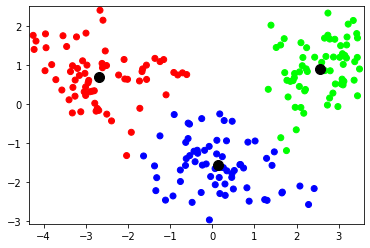
\includegraphics[width=0.75\textwidth]{Figures/K-means.png}
    \caption{Plot of the K-means cluster after PCA}
\end{figure}
